% define document class and set class options
\documentclass[11pt, a4paper]{article}

%===============================================
% *** LIST OF GENERAL PACKAGES *** %
% language package (french option available as well)
\usepackage[english]{babel}

% input fonts
\usepackage[utf8]{inputenc}
\usepackage[T1]{fontenc}
\usepackage{csquotes}


% customize default page geometry (size of margins, ...)
\usepackage{geometry}
\geometry{hmargin=2cm,vmargin=3cm}
\usepackage{titling}

\usepackage{titlesec}

% writing style
\usepackage{lmodern}
\usepackage{times}	 

% include images (image extensions & paths)
\usepackage{graphicx}
\DeclareGraphicsExtensions{.pdf,.jpg,.png,.eps}
\graphicspath{{figs/}}

\usepackage{wrapfig}

% display hyperlinks in the text
\usepackage{hyperref}  %
\hypersetup{colorlinks,%
            citecolor=red,%
            filecolor=black,%
            linkcolor=blue,%
            urlcolor=blue,%
            breaklinks=true}
            
% customize enumerated lists
\usepackage{enumitem}

% for \justify command
\usepackage{ragged2e}

% lipsum command to fill in the document (for visualisation purposes)
\usepackage{lipsum}

%===============================================
% *** CAPTIONS AND SUBFIGURES *** %
\usepackage{subcaption}

%===============================================
% *** TABLES *** %
\usepackage{booktabs}
\usepackage{multirow}

%=============================================== 
% *** BIBLIOGRAPHY (FOR BIBLATEX) *** %
\usepackage[
    backend=biber,
    style=numeric-comp
    ]{biblatex}


\usepackage{bookmark}
\addbibresource{bgtg_lib.bib}

% citation style: apa, ieee, authoryear, ...

%===============================================
% *** MATHS / PHYSICS PACKAGES *** %
\usepackage{amsfonts,amssymb,amsmath,amsthm}
\usepackage{mathrsfs}
\usepackage{mathtools}  % for DeclarePairedDelimiter
\usepackage{siunitx}    % notation physical units

% notations (shortcuts)
\newcommand{\bs}[1]{\boldsymbol{#1}}
\newcommand{\nbpix}{N}
\DeclareMathOperator{\prox}{prox}
\DeclareMathOperator{\sgn}{sgn}
\DeclareMathOperator*{\argmin}{argmin}
\DeclarePairedDelimiter{\norm}{\lVert}{\rVert}

%===============================================
% *** TITLE, AUTHOR AND DATE *** %
% \pretitle{\begin{center}\fontsize{30bp}{30bp}\selectfont}
% \posttitle{\par\end{center}}

% \preauthor{\begin{center}\fontsize{14bp}{14bp}\selectfont}
% \postauthor{\par\end{center}}
%===============================================
% *** MAIN DOCUMENT *** %
\begin{document}

\begin{titlepage}
\centering
% Logos
\begin{minipage}{.25\linewidth}
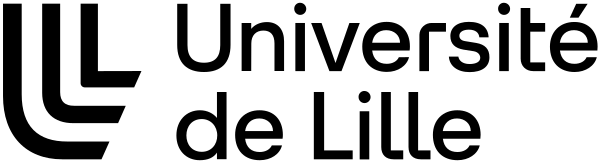
\includegraphics[width=\linewidth]{../images-figures/ulille.png}
\end{minipage}
\hfill
\begin{minipage}{.25\linewidth}
\centering

\includegraphics[width=\linewidth]{../images-figures/Centrale-Lille-Ecole.png}
\end{minipage}
\hfill
\begin{minipage}{.25\linewidth}

\includegraphics[width=\linewidth]{../images-figures/imt.png}
\end{minipage}

\vfill

% Subtitle

{\large Research project final report \\ \textit{March 2025} \vspace{1\baselineskip}}

% Title
\begin{minipage}{\linewidth}
\huge
\bfseries
\centering
\rule{\linewidth}{1.5pt}\\
Conditional Generation of Bass Guitar Tablature for Guitar Accompaniment in Western Popular Music\\[-3mm]
\rule{\linewidth}{1.5pt}
\end{minipage}

\vfill

% Persons involved 
\begin{minipage}{.45\linewidth}
\textit{Student:}\\
Olivier \textsc{Anoufa}\\
\textit{Data Science Master 2}

\end{minipage}
\hfill
\begin{minipage}{.45\linewidth}
\flushright
\textit{Supervisors:}\\
Alexandre \textsc{D'Hooge}\\
Ken \textsc{Déguernel}\\
\textit{Algomus team, CRIStAL}
\end{minipage}

\vfill

% Abstract
\begin{flushleft}
\justify
\textbf{Abstract ---} The field of symbolic music generation has seen great advancements with the rise of transformer-based architectures.
Addressing a specific need identified through a user study conducted on guitar players, we focus on developing AI tools to generate bass guitar tablatures conditioned on scores of other instruments in Western popular music.
The bass guitar, a crucial component of the rhythmic and harmonic sections in music, presents a unique challenge due to its dual role in providing structure and groove.
Building upon the tablature notation, the most popular way to share music among guitarists, this work adopts modern encoding schemes to integrate tablature representation into transformer-based models.
To this end, the project involves preprocessing a large dataset of music scores and fine-tuning state-of-the-art transformer architectures.
Due to the project being the first of its kind and its creative nature, the evaluation of the generated tablatures is mainly done qualitatively.
\vspace{.5\baselineskip}\\
\end{flushleft}
\vfill


% Period
% October 1st --- March 31st
% \vspace{1\baselineskip}\\
\begin{flushleft}
\textbf{Key-words ---} music information retrieval, conditional generation, guitar accompaniment, bass guitar, tablature;
\vspace{.5\baselineskip}\\
% \textbf{Mots-clés \hspace{1ex}---} effets audio, traitement de l'information musicale, traitement du signal différentiable, reproduction sonore, musique assistée par ordinateur.
\end{flushleft}
\vfill

% More logos
\begin{minipage}{.25\linewidth}

\includegraphics[height=3cm]{../images-figures/logoCRIStAL.png}
\end{minipage}
\hspace{7cm}
\begin{minipage}{.25\linewidth}

\includegraphics[height=3cm]{../images-figures/cnrs.png}
\end{minipage}

\end{titlepage}


% \begin{figure}[t]% We use titling to put a figure on top of the title page
%     \centering
%     
\includegraphics[width=.5\linewidth]{logos_empile}
% \end{figure}

% \title{Bass guitar tablature conditional generation for guitar accompaniment in western popular music}

% \author{Olivier \textsc{Anoufa} \\  University of Lille, France \\ Master 2 Data Science: Research project}

% {\let\newpage\relax\maketitle}

\newpage

\section{Introduction}

% Context and motivation
Natural language processing methods for the generation of symbolic music have experienced significant advancements in recent years.
The transformer architecture, first introduced for text by Vaswani et al. in 2017~\cite{vaswani_attention_2017}, has been later used to generate scores for various instruments, in diverse music genres~\cite{le_natural_2024}.
% REORGANIZE
A user study conducted by Bacot et al.~\cite{bacot_tablature_2025} showed a potential need for accompaniment generation tools for guitarists.
The questionnaire was answered by 31 guitarist-composers, and 7 of them followed up with an interview.
During the interviews, several guitarists answered that they would like to be able to generate bass guitar lines and drum parts without requiring familiarity with instruments.
Indeed, guitarists often resort to writing basic bass lines to accompany their compositions, and an AI tool could help by performing this functional task for them.

% Objectives
This need is the starting point for this project, proposed by the Algomus team, part of the CRIStAL laboratory.
We focus on the conditional aspect of symbolic music generation, for an instrument that has not been thoroughly studied yet: the bass guitar.
Specifically, the goal is to generate bass guitar tablatures given other instruments' scores, in the context of Western popular music.
Our objective is to try several combinations of conditioning instruments and to evaluate the quality of the generated tablatures both numerically and with the help of musicians.


% Terms definition (tablature, add the period when it was used)
% Difference between guitar and bass (role in the music)
To better understand what is at stake in this challenge, let us begin by precisely defining the terms of the subject and the role of the bass guitar in the context of Western popular music.
Since the human ear perceives low-frequency pulses more distinctly, the bass guitar is considered part of the rhythmic section of the band (together with the drums)~\cite{hove_superior_2014}.
However, the bass guitar also performs a harmonic — and sometimes melodic — role in the music, sustaining the lead instruments and adding groove to the composition.
Its adaptability makes the bass guitar a crucial component across various genres of Western popular music.


Learning score notation can be a daunting task for beginners, especially for string instruments like the guitar.
Historically, tablatures have been used since the Renaissance period as a simplified notation system for string instruments like the lute.
Originating around the 16th century, tablatures were an intuitive alternative to staff notation, allowing musicians to bypass the complexity of interpreting pitches.
This system explicitly linked symbols to physical actions on the instrument, such as pressing specific frets or strings.
In the 20th century, with the rise of internet forums and music sharing platforms, tablatures became a popular way to share music scores among amateur musicians.
First in ASCII format, tablatures were later digitalized and standardized in formats like GuitarPro\footnote{https://www.guitar-pro.com}, further extending their use for learning, practice, and composition in genres ranging from classical to popular music~\cite{sarmento_dadagp_2021}.
Tablatures originally did not contain rhythmic information, which is why they are generally combined with scores.
As a majority of guitarists learn many aspects of the songs they play by listening to them~\cite{green_how_2001},
tablatures are more of a prescriptive way to teach how to play a song that is already known by the musician.
Tablatures are part of what is called symbolic music, distinguished from audio music.
This project focuses on symbolic music, which corresponds to the written representation of music.
This representation can be in the form of scores or tablatures, but no audio will be involved in the generation process.


% FUNKO JAZZ, LENNY TRAVITZ, JACO PASTORIUS, VULFPECK
% add a fig Time is running out, melodic and rhythmic bass
\begin{figure}[!ht]
    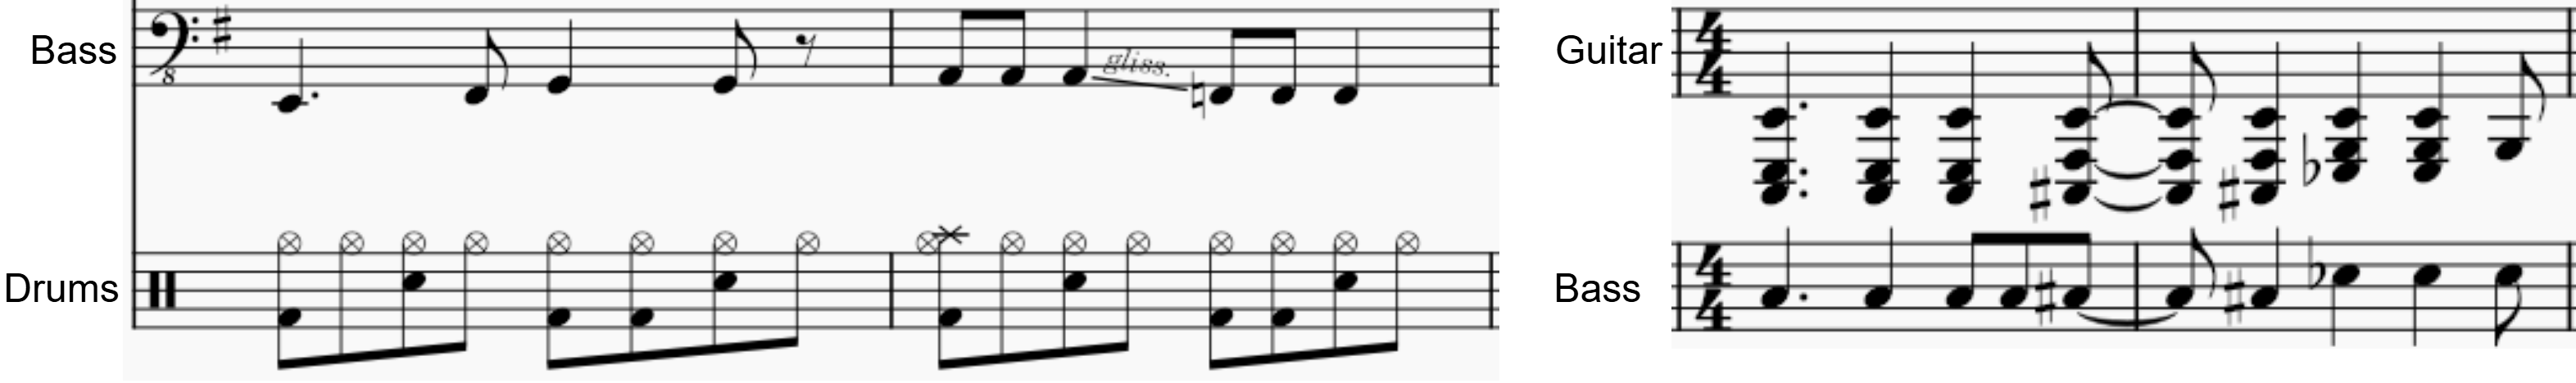
\includegraphics[width=.9\linewidth]{../images-figures/rhythmic_melodic.png}
    \caption{Rhythmic (left) and melodic (right) excerpts in Karma Police (left) and Everything in its Right Place (right) by Radiohead.}
    \label{fig:bass_tab_TIRO}
\end{figure}


Figure~\ref{fig:bass_tab_TIRO} shows a score excerpt of both a rhythmic and a melodic bass.
In the excerpt on the left, the bass guitar plays a rhythmic role, accompanying the drums in its pulsating rhythm 
whereas on the right, the bass guitar plays a melodic role, following the lead guitar's melody at a lower pitch.
In both these excerpts, the bass guitar is essential to the song's structure.
It adds grooves, harmonies and the low frequencies give the impression of a full sound.

Now that we have set the context and defined the terms, we will present the challenges we will face in generating bass guitar tablatures.
% Abstract challenges: (high-level such as: propose an informatic representation of music...)
Before tackling the task, we first need to retrieve and preprocess large datasets of music scores.
Then, we need to design a computational representation of music that is adapted to the task of generating bass guitar tablatures.
That is, a way to encode music scores in a meaningful way for the transformer architecture we will use.
Concerning the generation, we will start by leveraging state-of-the-art models but will adapt and tune them to the task at hand.

% GO DEEPER IN THE PRESENTATION TO AVOID TALKING ABOUT OUR WORK IN THE SOTA
More precisely, we will use the DadaGP dataset, which contains over 20 000 tablatures of Western popular music in GuitarPro format.
This data will be used to train an adapted version of the state of the art model in conditional generation proposed by Makris et al~\cite{makris_conditional_2022}.
Originally applied to generate drums parts conditionnally to the rest of the rhythmic section of the band (rhythmic guitar and bass guitar),
we will tune this model to generate bass guitar tablatures conditionnally different combinations of the other instruments of the band.
We detail the current state of the art in terms of data availability and conditional generation models in the next section.

\section{State of the art}

% Challenges (tokenization, conditional generation, attention, data cleaning), training of the model)
Adapting the transformer architecture — originally developed for text processing — to symbolic music presents many challenges.
Symbolic music datasets, unlike text corpus, are limited in both size and diversity, posing challenges for training robust models\cite{le_natural_2024}.
Tokenization must be tailored to represent pitch, duration, and dynamics, while attention mechanisms require adaptation to capture the hierarchical and temporal structure of music.
Finally, data cleaning and preprocessing steps are critical to standardize music scores and ensure the compatibility with sequence models.

% State of the art (survey, DadaGP, Compound Gen, Structure-informed positional encoding, gen coherent drum accompaniment)
% ResearchRabbit to find potential other articles

\subsection{Data availability}


Symbolic music datasets are a cornerstone for training deep learning models, yet their availability and quality significantly vary across domains.
In music composition and generation, datasets are often limited in size and diversity, especially when compared to text or image datasets.
For bass guitar tablatures, the challenge is even more pronounced due to the niche nature of the instrument and the focus on other instruments in existing datasets.


The MIDI standard has dominated symbolic music datasets for decades, allowing the development of resources like the Lakh MIDI dataset and MAESTRO dataset.
However, while these datasets offer general-purpose symbolic music, they lack the specificity required for tasks involving tablatures or instrument-specific representation.
The GuitarSet dataset, for example, focuses on acoustic guitar transcription but does not provide sufficient symbolic information for bass guitar.
Similarly, the DadaGP dataset addresses the need for multi-instrument symbolic music data in tablature format, but its emphasis is on rock and metal genres, which limits the diversity of bass guitar styles\cite{sarmento_dadagp_2021}.


Bass guitar data, especially in tablature format, suffers from a lack of standardization and availability.
Tablature files are often stored in private formats like GuitarPro or as non-standardized text files, making it challenging to preprocess them for machine learning tasks\cite{sarmento_dadagp_2021}.
Moreover, rhythm and dynamics, critical elements in bass guitar playing, are frequently absent in publicly available tablatures, complicating their utility in generative tasks.


Efforts like DadaGP illustrate the potential of GuitarPro files repositoriess to create symbolic datasets that include bass guitar parts.
Moreover DadaGP also provides a tokenized format inspired by MIDI encodings, offering a foundation for training sequence models.
On the other hand, pre-trained models on broader datasets like MAESTRO or Lakh MIDI can be fine-tuned on smaller datasets, reducing the dependency on large volumes of task-specific data\cite{makris_conditional_2022, sarmento_dadagp_2021}.
For our project, we use the DadaGP dataset. Its very specific tokenization will be discussed in the next section.


\subsection{Tokenization}

Tokenization in the context of deep learning music generation has been discussed by several previous works\cite{agarwal_structure-informed_2024, makris_conditional_2022, sarmento_dadagp_2021, hsiao_compound_2021, cournut_encodages_2020}.

% General overview of the possible startegies (NLP survey)
Tokenization in music involves converting complex musical content into a sequence of elements that can be processed computationally.
Much like tokenization in natural language processing (NLP), it breaks down music into manageable units, though in music, the focus is on musical features like pitch, duration, and velocity.
In symbolic music information retrieval (MIR), tokenization strategies are generally classified into two categories: time-slice-based and event-based. 
Time-slice-based tokenization divides music into fixed-time intervals, such as 16th notes, which can be represented in formats like piano rolls or multi-hot vectors, capturing simultaneous notes at each time slice.
Event-based tokenization, on the other hand, focuses on specific musical events, such as a note being played or a measure starting, often using formats like MIDI, which encode music as a series of events.
This approach can involve elementary tokens, which represent individual features like pitch or duration, or composite tokens that aggregate multiple features into one token, providing a more compact representation.
Notably, tokenization strategies like REMI (Revamped MIDI-derived events) and MIDI-like tokenization allow for consistent representation of rhythmic and pitch elements while addressing complexities like polyphony and multiple tracks in multi-instrument music\cite{le_natural_2024, cournut_encodages_2020}.


% DadaGP tokenization
The DadaGP tokenization format adopts an event-based approach, similar to other music generation models, by representing musical events as discrete tokens.
It uses a Python script with PyGuitarPro to convert GuitarPro files into a tokenized sequence, beginning with metadata tokens such as artist, downtune, tempo, and start.
Pitched instrument notes are encoded with a combination of tokens representing instrument, note, string, and fret, while rests are denoted with a separate token structure.
For drumset sounds, a specific tokenization scheme using MIDI percussion maps is employed, where each drum sound is represented by a unique token (e.g., drums:note:36 for a kick drum).
The system also uses wait tokens to separate notes and rests, enabling the model to infer note durations without the need for explicit note-off tokens.
This approach ensures that new notes automatically silence previous ones, except in cases where ghost notes or let-ring effects are involved.
Additionally, the tokenization format records changes in musical structure, such as new measures, tempo shifts, and note effects, with each change being represented as a distinct token.
However, the tokenization does not encode dynamics or articulations. These are supposed to be inferred by the user after generation.


\begin{figure}[h!]
    \centering
    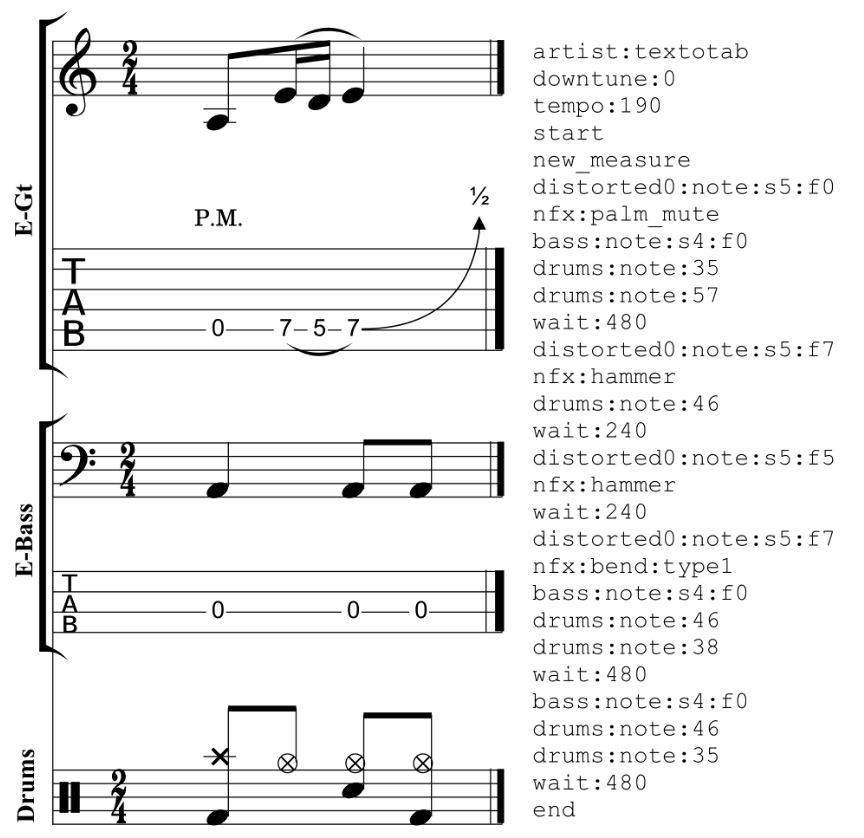
\includegraphics[width=.5\linewidth]{../images-figures/dadagp_tokenization_example_measure.png}
    \caption{Example measure with a distorted guitar, bass and drums in GuitarPro’s graphical user interface (left), and its conversion into token format (right). Figure taken from \cite{sarmento_dadagp_2021}}
    \label{fig:dadagp_tokenization}
\end{figure}


Figure \ref{fig:dadagp_tokenization} illustrates the tokenization process for a measure in a GuitarPro file, showing the conversion of a musical event into a tokenized sequence.
We notice the three first tokens are the metadata tokens. "start" token marks the beginning of the song.
Afterwards, each measure is announced by a "new\_measure" token.
In between, the instruments' notes are encoded using the tablature notation for the guitars.
For instance the first note played here is distorted0:note:s5:f0 (string 5, fret 0).
It is followed by a nfx token "nfx:palm\_mute", which is a note effect token that applies to the previous note.
Finally, the duration of the note is given by the wait token "wait:480" (480 ticks in GuitarPro correspond to an eighth note).
If no tokens of a specific instrument are present between two wait tokens, it means that the instrument keeps on playing the same note.
This is the case of the bass in the example.
Its first quarter note lasts for 960 ticks, therefore we have to look after the three first wait tokens (480 + 240 + 240) before seeing a new token for the bass.


% Compound Gen tokenization
As we plan to use the model built by Makris et al. in 2022, we will also consider the tokenization they used.
The proposed tokenization model introduces a compound word (CP) representation, inspired by previous CP-based approaches\cite{hsiao_compound_2021}.
Unlike traditional tokenization strategies such as MIDI-like or REMI, which encode music as a linear sequence of tokens, CP groups multiple features of a musical event into a single "super token" or "word".
This n-dimensional representation significantly reduces sequence length and improves computational efficiency in Transformer-based architectures\cite{makris_conditional_2022}.


In this model, the CP representation is adapted for an Encoder-Decoder architecture to condition drum generation on accompanying rhythm tracks, such as bass and guitar.
The Encoder processes a 5-dimensional CP representation that includes rhythm track features and high-level musical information like tempo and time signature, which are known to influence the complexity and density of drum tracks.
Both the Encoder and Decoder adopt bar-based segmentation, consistent with existing CP and REMI representations.
By combining rhythm section inputs and high-level parameters, this tokenization approach aligns with the fundamental musical principles of contemporary western music's rhythm section\cite{makris_conditional_2022}.
As said previously, our work will use the DadaGP tokenization. However, the nature of the generation task we want to perform is very similar to the one of Makris et al. in the sense that bass guitar and drums are part of the same rhythm section.


\begin{figure}[h!]
    \centering
    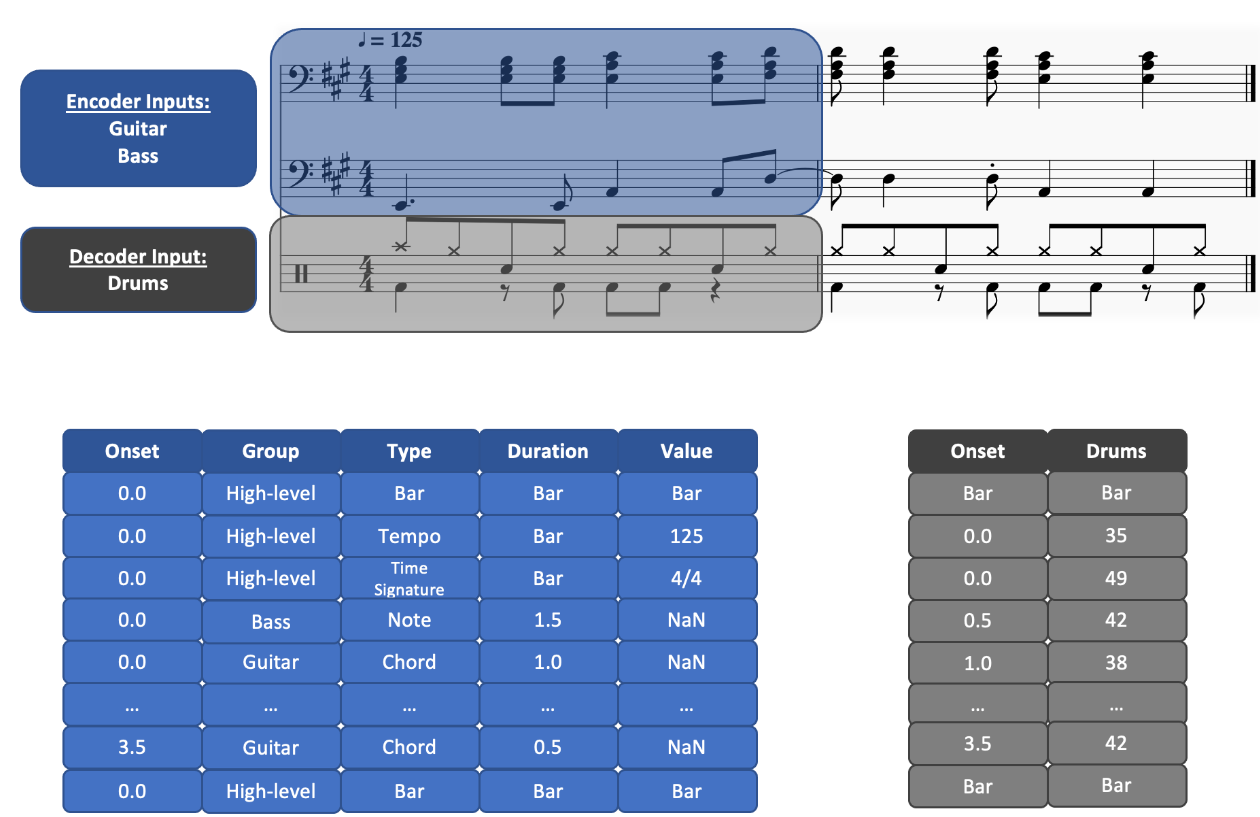
\includegraphics[width=.5\linewidth]{../images-figures/tokenization_makris.png}
    \caption{Example of a CP representation used for training. Figure taken from \cite{makris_conditional_2022}}
    \label{fig:compound_gen_tokenization}
\end{figure}


Figure \ref{fig:compound_gen_tokenization} shows an example of a CP representation used for training in the model developed by Makris et al.
We notice that the rhythmic section, composed of a rhythmic guitar and a bass (in blue on the figure), constitutes the conditioning part of the model.
Their representation as tokens encode the duration and type of the notes played, but not the pitch of the notes as it is not relevant for the drum generation task.
In grey, the drum part's encoding excludes all information about velocities and duration.
Drums notes and are only represented by their onset in the bar and the drum component played.

\subsection{Conditional generation models}

% Intro about conditional generation using control tokens (prompt tokens)
% --> GTR CTRL, ShredGP, ProgGP
Our first idea was to use the GuitarCTRL model developed by Sarmento et al. in 2021\cite{sarmento_gtr-ctrl_2023}.
The GTR CTRL model utilizes a Transformer-XL architecture\cite{dai_transformer-xl_2019}, which improves on the vanilla Transformer by introducing recurrence and modified positional encodings, enabling long-term dependency learning.
This model includes two key control types: instrumentation (inst-CTRL) and genre (genre-CTRL).
For instrumentation, tokens marking the start and end of each instrument are inserted into the header, guiding the model to generate music for specified instruments, such as bass and drums or distorted guitar and drums.
Genre control tokens are similarly placed at the beginning of the sequence, with a dataset covering over 200 songs per genre, including Metal, Rock, Punk, Folk, and Classical.
The model uses various prompts at inference, ranging from full-prompt (including two measures plus the genre token) to empty-prompt (only the genre token).
This model was used to generate a baseline result for our project, conditioning the generation to bass guitar only.


% Start with a historic of BI-LSTM in NLP (2015)
% Dive in makris et al model (BiLSTM) (SOTA in drum generation)
The model we wish to use for our project is the one developed by Makris et al. in 2022\cite{makris_conditional_2022}.
It employs an Encoder-Decoder architecture with a BiLSTM Encoder and a Transformer Decoder utilizing Relative Global Attention.
The Encoder is made of several BiLSTM layers. It processes Compound Representation (CP) inputs to generate a latent variable z that encodes high-level features of the input and conditional tracks.
BiLSTM (Bidirectional Long Short-Term Memory) were first introduced by Graves et al. in 2005\cite{graves_framewise_2005}. It is a type of recurrent neural network (RNN) that processes data in both forward and backward directions.
This allows the model to consider both past (previous time steps) and future (upcoming time steps) context in the sequence
The Decoder consists of self-attention layers and feed-forward layers. 
It combines z with previous timestep embeddings to predict drum onsets and pitches.



The model uses input sizes that are different from the ones we may use with our tokenization.
However we are interested in the ability of the model to generate conditionnally throughout the whole sequence.
In comparison, GTR CTRL only conditions the generation at the beginning of the sequence.
One of the issue we encountered when generating bass guitar was that other instruments ended up being generated further in the sequence.
To avoid this we tried setting the probability of predicting tokens from any other instruments to 0, but even then the bass lines generated were not coherent.
This model is simply not suited for our task which explains our motivations to adapt the BiLSTM model.


\section{Data preprocessing}

% What we have done (data preprocessing, getting the rhythmic instrument, retrieving the tokens, baseline using dadagp (GuitarCTRL))
\subsection{DadaGP token processing}
% --> Retrieving, cleaning, mapping DadaGP
% Rhythmic guitar detection (cite paper)

The DadaGP dataset provides token files containing information for all instruments in a score.
As we want to explore various conditioning combinations for tablature generation, we developed a function to extract tokens specific to selected instruments.
We considered several possible ways to perform this extraction: runnning DadaGP's token processing script for each instrument, or filtering the tokens from the complete token text file based on the instrument name.
Opening, parsing and looping on the GuitarPro file using pygp is needed for the DadaGP token processing script and is very time-consuming, much more than processing txt files.
We recall that DadaGP comprises 26,181 GuitarPro files. Using our algorithm it only took 5min30 to process all the files and generate the token files with the bass guitar tokens only.
To perform this operation, we leverage the fact that tokens of a given instrument start with the instrument name followed by a colon, e.g., \texttt{bass:} for the bass guitar.
However we must be careful not to miss the potential note effect tokens that are not instrument-specific, but come right after the token they are related to.
After extracting those tokens and the general tokens (metadata tokens and wait tokens),
we sum the potential consecutive wait tokens that were previously separated by notes from instruments that are no longer present.
An example of token extraction is shown in Figure~\ref{fig:token_list}.

\begin{figure}[!ht]
    \centering
    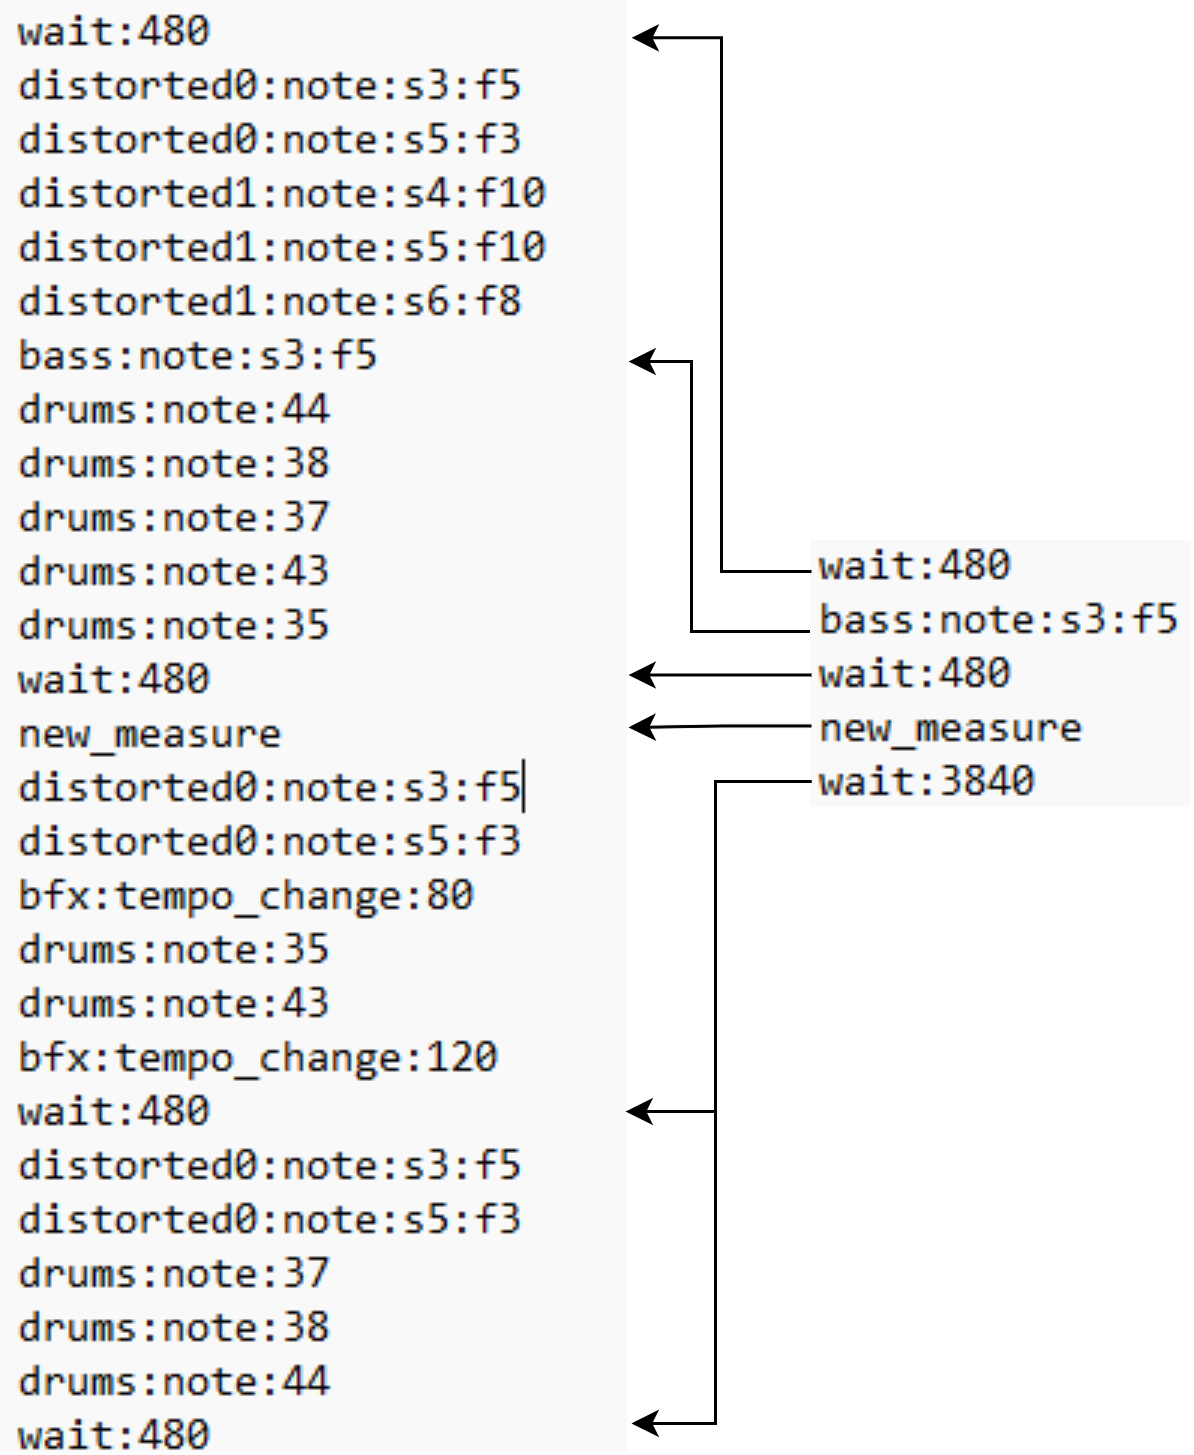
\includegraphics[width=.5\linewidth]{../images-figures/token_extraction.png}
    \caption{Example of an extraction of bass guitar token in The Strokes - Last Nite}
    \label{fig:token_extraction}
\end{figure}

An example of token extraction is shown in Figure~\ref{fig:token_extraction}.
This figure also shows the concatenation of wait tokens.
At the end of the song, the bass guitar stops playing before the other instruments.
We can notice the several \texttt{wait:480} tokens that are summed up to a single \texttt{wait:3840} token.


\subsection{Rythmic guitar identification}

The algorithm we just presented allows us to extract tokens for any instrument in the DadaGP dataset.
We then focused on conditioning bass guitar tablature generation using the rhythmic guitar.
In typical rock band instrumentation, rhythmic guitars complement bass guitars with their repetitive chord patterns, providing harmonic and rhythmic structure at a higher pitch \cite{regnier_identification_2021}.
This characteristic makes them particularly relevant for conditioning bass generation tasks.

To identify rhythmic guitar parts in the DadaGP dataset, we implemented the method proposed by Régnier et al. \cite{regnier_identification_2021},
which uses features describing notes and chords at the bar level, along with corresponding tablatures.
Their model outputs a prediction between 0 and 1 for each bar. The closest to 1, the more likely the part is a lead on the bar, and the closest to 0, the more likely it is a rhythmic guitar part on the bar.
In their paper, they consider that a score below 0.5 correspond to a rhythmic guitar parts. We wanted to select and condition the generation on only one rhythmic guitar part, the "most" rhythmic.
Therefore, we applied the 0.5 threshold to the predictions and selected the part with the highest proportion of rhythmic bar over the course of the song.
Implementing this method required adapting their code to the DadaGP dataset.
Significant effort was spent mapping the identified rhythmic guitar parts to their respective names in the DadaGP files, as the dataset renames instruments, whereas the identification tool relies on GuitarPro part names.

\section{Baseline predictions}

With the preprocessed data, we began by establishing a baseline model for bass guitar tablature generation.
Initially, we utilized a pre-trained checkpoint from the DadaGP paper \cite{sarmento_dadagp_2021} without additional training.

To generate bass-specific outputs, we experimented with various prompts.
First, we provided a single bass guitar note as the initial token, however the model quickly incorporated tokens from other instruments.
This is an issue documented in the GuitarCTRL paper\cite{sarmento_gtr-ctrl_2023} where they used a metric called the UIP score (Unpromped Instrument Presence) to evaluate the model's ability to generate a specific combinations of instruments.
To constrain the output to bass tokens, we modified the logits of non-bass instruments by setting them to $-\infty$.

% FIGURE REPETITIVE GENERATION
\begin{figure}[!ht]
    \centering
    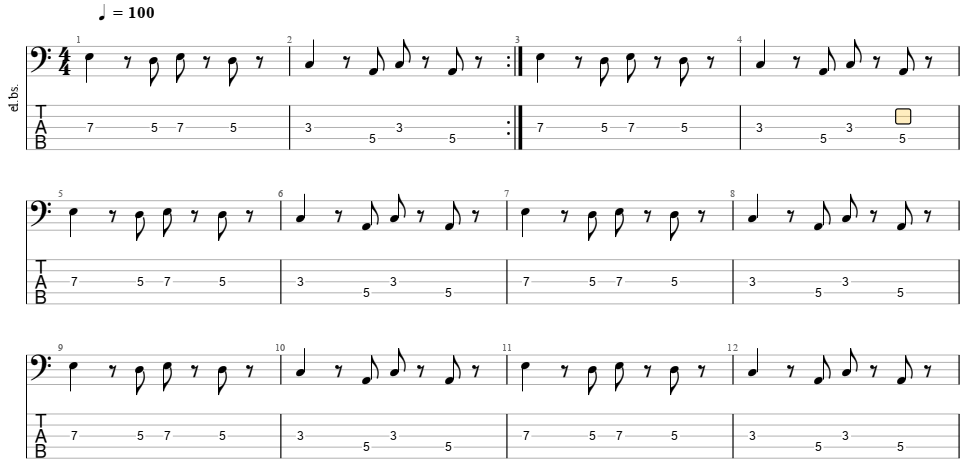
\includegraphics[width=.75\linewidth]{../images-figures/generated_bass_baseline.png}
    \caption{Example of a bass generation from the baseline model}
    \label{fig:repetitive_generation}
\end{figure}

An example of a bass tablature generated this way is shown in Figure~\ref{fig:repetitive_generation}.
While this forced the model to generate only bass tokens, the output quality was poor, featuring repetitive phrases, harmonically incorrect notes, or complete aberrations.
This was expected, as the model was not trained explicitly for bass only generation. 
Unfortunately, we cannot provide a quantitative evaluation of the generated tablatures, as we have not yet defined an evaluation metric.

\section{Workplan}
% Workplan (what we are going to do)

% DETAILS
Our next steps include:
\begin{enumerate}
    \item Propose an evaluation metric to quantify the quality of the generated tablatures.
    \item Understand the code of the model proposed by Makris et al. using their Github repository.
    \item Adapt the model to our task and our data.
    \item Generate predictions with conditional information from several combinations of instruments.
\end{enumerate}

\newpage

%\nocite{*} % force display of the full content of the .bib file, w/o any citation in the document
\printbibliography% references: print bibliography (with bibtex file)

\end{document}